\documentclass[twoside]{book}

% Packages required by doxygen
\usepackage{fixltx2e}
\usepackage{calc}
\usepackage{doxygen}
\usepackage[export]{adjustbox} % also loads graphicx
\usepackage{graphicx}
\usepackage[utf8]{inputenc}
\usepackage{makeidx}
\usepackage{multicol}
\usepackage{multirow}
\PassOptionsToPackage{warn}{textcomp}
\usepackage{textcomp}
\usepackage[nointegrals]{wasysym}
\usepackage[table]{xcolor}

% Font selection
\usepackage[T1]{fontenc}
\usepackage[scaled=.90]{helvet}
\usepackage{courier}
\usepackage{amssymb}
\usepackage{sectsty}
\renewcommand{\familydefault}{\sfdefault}
\allsectionsfont{%
  \fontseries{bc}\selectfont%
  \color{darkgray}%
}
\renewcommand{\DoxyLabelFont}{%
  \fontseries{bc}\selectfont%
  \color{darkgray}%
}
\newcommand{\+}{\discretionary{\mbox{\scriptsize$\hookleftarrow$}}{}{}}

% Page & text layout
\usepackage{geometry}
\geometry{%
  a4paper,%
  top=2.5cm,%
  bottom=2.5cm,%
  left=2.5cm,%
  right=2.5cm%
}
\tolerance=750
\hfuzz=15pt
\hbadness=750
\setlength{\emergencystretch}{15pt}
\setlength{\parindent}{0cm}
\setlength{\parskip}{3ex plus 2ex minus 2ex}
\makeatletter
\renewcommand{\paragraph}{%
  \@startsection{paragraph}{4}{0ex}{-1.0ex}{1.0ex}{%
    \normalfont\normalsize\bfseries\SS@parafont%
  }%
}
\renewcommand{\subparagraph}{%
  \@startsection{subparagraph}{5}{0ex}{-1.0ex}{1.0ex}{%
    \normalfont\normalsize\bfseries\SS@subparafont%
  }%
}
\makeatother

% Headers & footers
\usepackage{fancyhdr}
\pagestyle{fancyplain}
\fancyhead[LE]{\fancyplain{}{\bfseries\thepage}}
\fancyhead[CE]{\fancyplain{}{}}
\fancyhead[RE]{\fancyplain{}{\bfseries\leftmark}}
\fancyhead[LO]{\fancyplain{}{\bfseries\rightmark}}
\fancyhead[CO]{\fancyplain{}{}}
\fancyhead[RO]{\fancyplain{}{\bfseries\thepage}}
\fancyfoot[LE]{\fancyplain{}{}}
\fancyfoot[CE]{\fancyplain{}{}}
\fancyfoot[RE]{\fancyplain{}{\bfseries\scriptsize Generated by Doxygen }}
\fancyfoot[LO]{\fancyplain{}{\bfseries\scriptsize Generated by Doxygen }}
\fancyfoot[CO]{\fancyplain{}{}}
\fancyfoot[RO]{\fancyplain{}{}}
\renewcommand{\footrulewidth}{0.4pt}
\renewcommand{\chaptermark}[1]{%
  \markboth{#1}{}%
}
\renewcommand{\sectionmark}[1]{%
  \markright{\thesection\ #1}%
}

% Indices & bibliography
\usepackage{natbib}
\usepackage[titles]{tocloft}
\setcounter{tocdepth}{3}
\setcounter{secnumdepth}{5}
\makeindex

% Hyperlinks (required, but should be loaded last)
\usepackage{ifpdf}
\ifpdf
  \usepackage[pdftex,pagebackref=true]{hyperref}
\else
  \usepackage[ps2pdf,pagebackref=true]{hyperref}
\fi
\hypersetup{%
  colorlinks=true,%
  linkcolor=blue,%
  citecolor=blue,%
  unicode%
}

% Custom commands
\newcommand{\clearemptydoublepage}{%
  \newpage{\pagestyle{empty}\cleardoublepage}%
}

\usepackage{caption}
\captionsetup{labelsep=space,justification=centering,font={bf},singlelinecheck=off,skip=4pt,position=top}

%===== C O N T E N T S =====

\begin{document}

% Titlepage & ToC
\hypersetup{pageanchor=false,
             bookmarksnumbered=true,
             pdfencoding=unicode
            }
\pagenumbering{alph}
\begin{titlepage}
\vspace*{7cm}
\begin{center}%
{\Large My Project }\\
\vspace*{1cm}
{\large Generated by Doxygen 1.8.14}\\
\end{center}
\end{titlepage}
\clearemptydoublepage
\pagenumbering{roman}
\tableofcontents
\clearemptydoublepage
\pagenumbering{arabic}
\hypersetup{pageanchor=true}

%--- Begin generated contents ---
\chapter{Hierarchical Index}
\section{Class Hierarchy}
This inheritance list is sorted roughly, but not completely, alphabetically\+:\begin{DoxyCompactList}
\item \contentsline{section}{Combine}{\pageref{class_combine}}{}
\item \contentsline{section}{fts}{\pageref{classfts}}{}
\item Q\+G\+L\+Widget\begin{DoxyCompactList}
\item \contentsline{section}{G\+L\+Widget}{\pageref{class_g_l_widget}}{}
\end{DoxyCompactList}
\item Q\+Main\+Window\begin{DoxyCompactList}
\item \contentsline{section}{Main\+Window}{\pageref{class_main_window}}{}
\end{DoxyCompactList}
\item \contentsline{section}{qt\+\_\+meta\+\_\+stringdata\+\_\+\+G\+L\+Widget\+\_\+t}{\pageref{structqt__meta__stringdata___g_l_widget__t}}{}
\item \contentsline{section}{qt\+\_\+meta\+\_\+stringdata\+\_\+\+Main\+Window\+\_\+t}{\pageref{structqt__meta__stringdata___main_window__t}}{}
\item \contentsline{section}{temp\+\_\+threed\+\_\+object}{\pageref{classtemp__threed__object}}{}
\item \contentsline{section}{threed\+\_\+object}{\pageref{classthreed__object}}{}
\item \contentsline{section}{threedplane}{\pageref{classthreedplane}}{}
\item \contentsline{section}{Ui\+\_\+\+Main\+Window}{\pageref{class_ui___main_window}}{}
\begin{DoxyCompactList}
\item \contentsline{section}{Ui\+:\+:Main\+Window}{\pageref{class_ui_1_1_main_window}}{}
\end{DoxyCompactList}
\end{DoxyCompactList}

\chapter{Class Index}
\section{Class List}
Here are the classes, structs, unions and interfaces with brief descriptions\+:\begin{DoxyCompactList}
\item\contentsline{section}{\mbox{\hyperlink{classthreed__object}{threed\+\_\+object}} }{\pageref{classthreed__object}}{}
\item\contentsline{section}{\mbox{\hyperlink{class_v_i_e_w}{V\+I\+EW}} }{\pageref{class_v_i_e_w}}{}
\end{DoxyCompactList}

\chapter{Class Documentation}
\hypertarget{class_combine}{}\section{Combine Class Reference}
\label{class_combine}\index{Combine@{Combine}}
\subsection*{Public Attributes}
\begin{DoxyCompactItemize}
\item 
\mbox{\Hypertarget{class_combine_a6a910528bedd4c33f36b313c69657cc0}\label{class_combine_a6a910528bedd4c33f36b313c69657cc0}} 
std\+::vector$<$ std\+::vector$<$ float $>$ $>$ {\bfseries edge}
\end{DoxyCompactItemize}


The documentation for this class was generated from the following file\+:\begin{DoxyCompactItemize}
\item 
global.\+h\end{DoxyCompactItemize}

\hypertarget{classfts}{}\section{fts Class Reference}
\label{classfts}\index{fts@{fts}}
\subsection*{Public Attributes}
\begin{DoxyCompactItemize}
\item 
\mbox{\Hypertarget{classfts_a7295fb27e8b87209e4be4bc116a99013}\label{classfts_a7295fb27e8b87209e4be4bc116a99013}} 
std\+::vector$<$ std\+::vector$<$ float $>$ $>$ {\bfseries fvertex}
\item 
\mbox{\Hypertarget{classfts_a4cf1248686c273f9c517d210015fa0c1}\label{classfts_a4cf1248686c273f9c517d210015fa0c1}} 
std\+::vector$<$ std\+::vector$<$ float $>$ $>$ {\bfseries tvertex}
\item 
\mbox{\Hypertarget{classfts_a28ca005657153a7052d512b558ebd9ac}\label{classfts_a28ca005657153a7052d512b558ebd9ac}} 
std\+::vector$<$ std\+::vector$<$ float $>$ $>$ {\bfseries svertex}
\item 
\mbox{\Hypertarget{classfts_a7aec6b15df57f1dc4b62ca1a7ff23956}\label{classfts_a7aec6b15df57f1dc4b62ca1a7ff23956}} 
std\+::vector$<$ std\+::vector$<$ float $>$ $>$ {\bfseries fedge}
\item 
\mbox{\Hypertarget{classfts_aad0108365ca7bf36d771c416c15ec50a}\label{classfts_aad0108365ca7bf36d771c416c15ec50a}} 
std\+::vector$<$ std\+::vector$<$ float $>$ $>$ {\bfseries tedge}
\item 
\mbox{\Hypertarget{classfts_ab93187bdd5b15efb308195c460c57070}\label{classfts_ab93187bdd5b15efb308195c460c57070}} 
std\+::vector$<$ std\+::vector$<$ float $>$ $>$ {\bfseries sedge}
\end{DoxyCompactItemize}


The documentation for this class was generated from the following file\+:\begin{DoxyCompactItemize}
\item 
global.\+h\end{DoxyCompactItemize}

\hypertarget{class_g_l_widget}{}\section{G\+L\+Widget Class Reference}
\label{class_g_l_widget}\index{G\+L\+Widget@{G\+L\+Widget}}
Inheritance diagram for G\+L\+Widget\+:\begin{figure}[H]
\begin{center}
\leavevmode
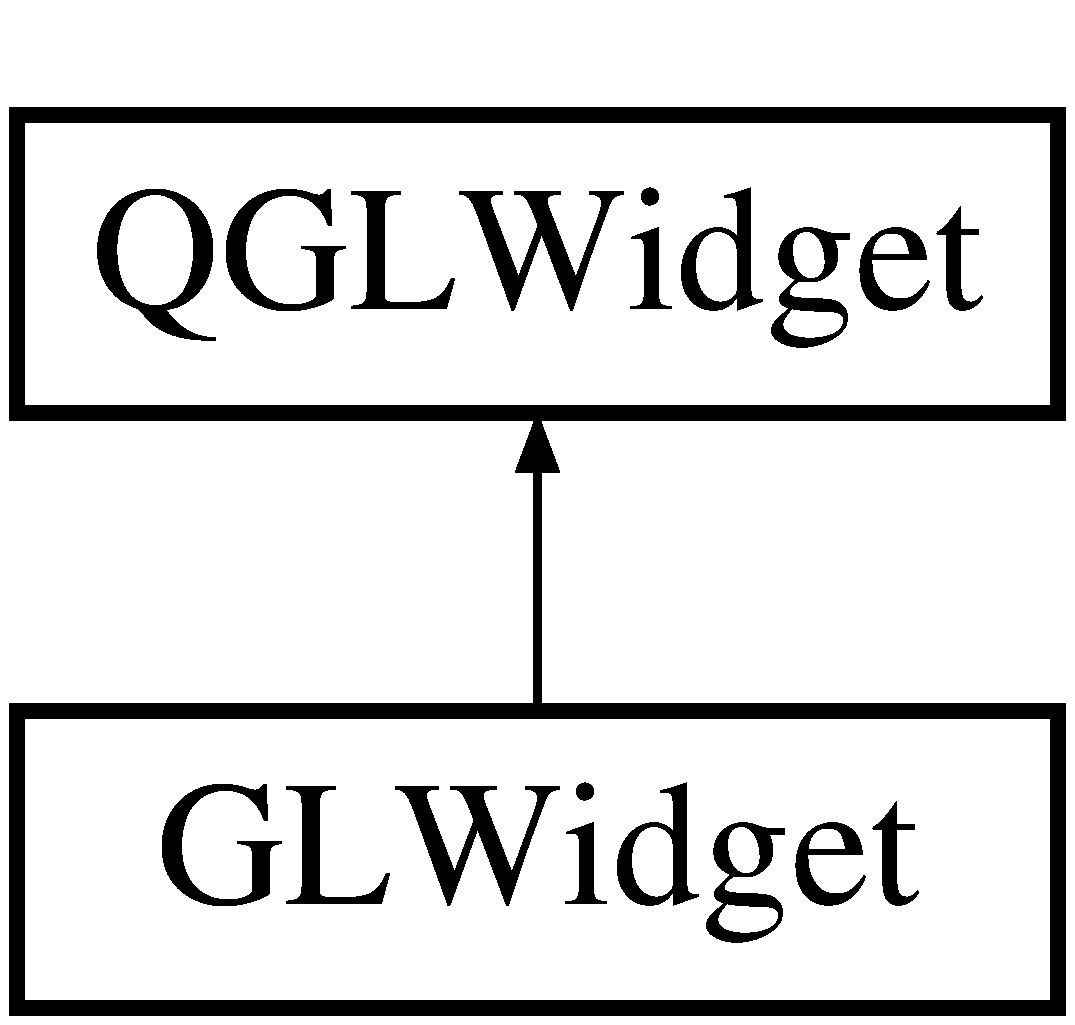
\includegraphics[height=2.000000cm]{class_g_l_widget}
\end{center}
\end{figure}
\subsection*{Public Member Functions}
\begin{DoxyCompactItemize}
\item 
\mbox{\Hypertarget{class_g_l_widget_ab79c391c86de1ffb76f6950b49d82c0c}\label{class_g_l_widget_ab79c391c86de1ffb76f6950b49d82c0c}} 
{\bfseries G\+L\+Widget} (Q\+Widget $\ast$parent=0)
\item 
\mbox{\Hypertarget{class_g_l_widget_a7fab13e8cc9fc0730ca54c08b2c923a7}\label{class_g_l_widget_a7fab13e8cc9fc0730ca54c08b2c923a7}} 
void {\bfseries initialize\+GL} ()
\item 
\mbox{\Hypertarget{class_g_l_widget_a640b5570cb2b37724fd5b58a77339c5e}\label{class_g_l_widget_a640b5570cb2b37724fd5b58a77339c5e}} 
void {\bfseries paint\+GL} ()
\item 
\mbox{\Hypertarget{class_g_l_widget_a5e960cecb41f3937742f76a0a9103c88}\label{class_g_l_widget_a5e960cecb41f3937742f76a0a9103c88}} 
void {\bfseries resize\+GL} (int w, int h)
\end{DoxyCompactItemize}


The documentation for this class was generated from the following files\+:\begin{DoxyCompactItemize}
\item 
glwidget.\+h\item 
glwidget.\+cpp\end{DoxyCompactItemize}

\hypertarget{class_ui_1_1_main_window}{}\section{Ui\+:\+:Main\+Window Class Reference}
\label{class_ui_1_1_main_window}\index{Ui\+::\+Main\+Window@{Ui\+::\+Main\+Window}}
Inheritance diagram for Ui\+:\+:Main\+Window\+:\begin{figure}[H]
\begin{center}
\leavevmode
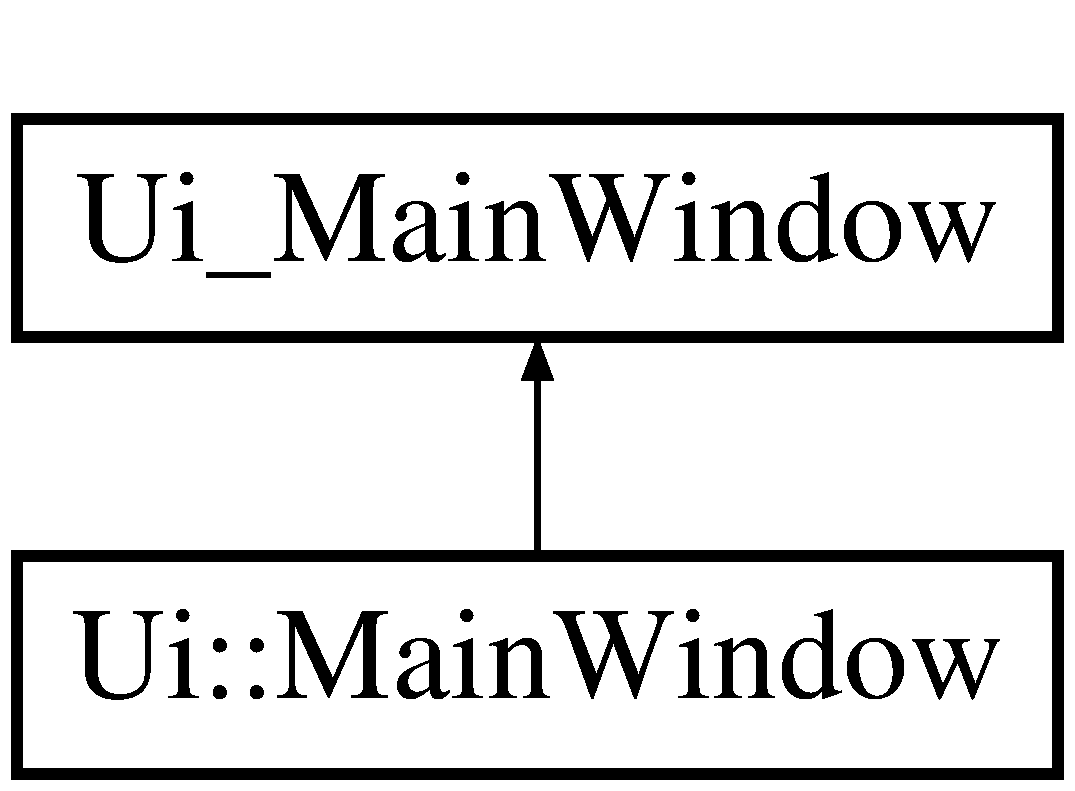
\includegraphics[height=2.000000cm]{class_ui_1_1_main_window}
\end{center}
\end{figure}
\subsection*{Additional Inherited Members}


The documentation for this class was generated from the following file\+:\begin{DoxyCompactItemize}
\item 
ui\+\_\+mainwindow.\+h\end{DoxyCompactItemize}

\hypertarget{class_main_window}{}\section{Main\+Window Class Reference}
\label{class_main_window}\index{Main\+Window@{Main\+Window}}
Inheritance diagram for Main\+Window\+:\begin{figure}[H]
\begin{center}
\leavevmode
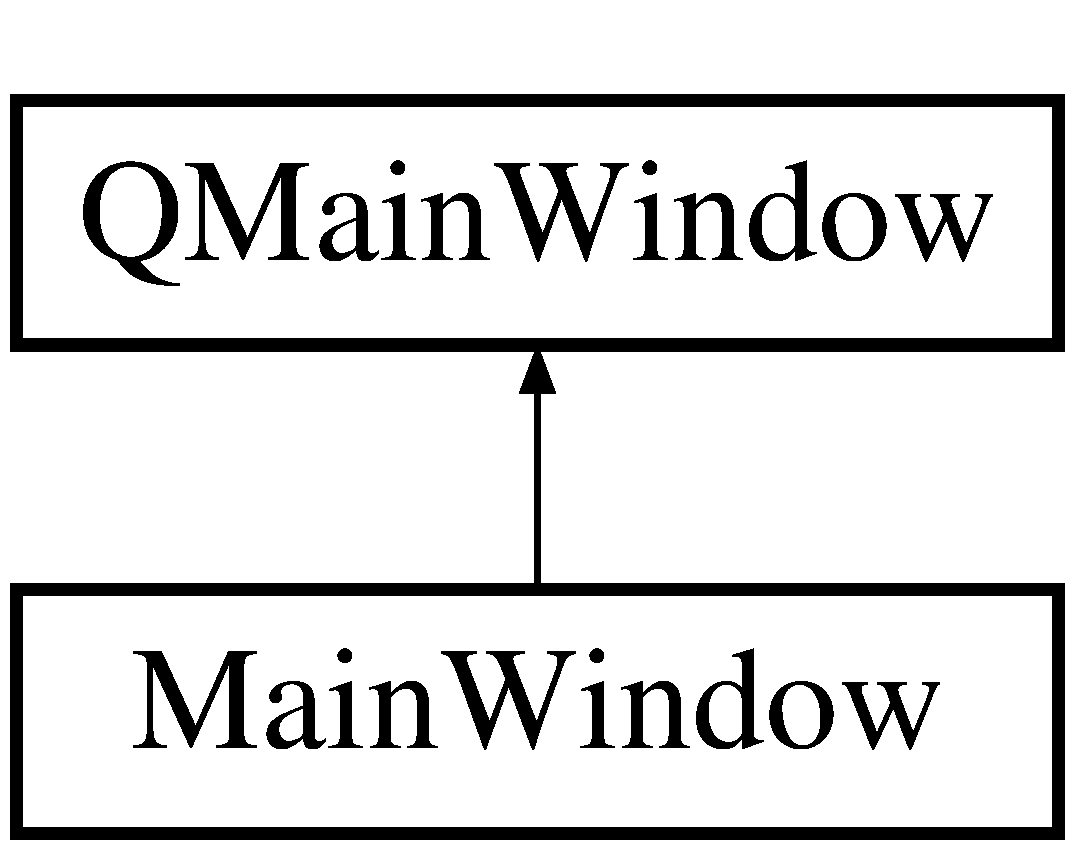
\includegraphics[height=2.000000cm]{class_main_window}
\end{center}
\end{figure}
\subsection*{Public Member Functions}
\begin{DoxyCompactItemize}
\item 
\mbox{\Hypertarget{class_main_window_a8b244be8b7b7db1b08de2a2acb9409db}\label{class_main_window_a8b244be8b7b7db1b08de2a2acb9409db}} 
{\bfseries Main\+Window} (Q\+Widget $\ast$parent=0)
\end{DoxyCompactItemize}


The documentation for this class was generated from the following files\+:\begin{DoxyCompactItemize}
\item 
mainwindow.\+h\item 
mainwindow.\+cpp\end{DoxyCompactItemize}

\hypertarget{structqt__meta__stringdata___g_l_widget__t}{}\section{qt\+\_\+meta\+\_\+stringdata\+\_\+\+G\+L\+Widget\+\_\+t Struct Reference}
\label{structqt__meta__stringdata___g_l_widget__t}\index{qt\+\_\+meta\+\_\+stringdata\+\_\+\+G\+L\+Widget\+\_\+t@{qt\+\_\+meta\+\_\+stringdata\+\_\+\+G\+L\+Widget\+\_\+t}}
\subsection*{Public Attributes}
\begin{DoxyCompactItemize}
\item 
\mbox{\Hypertarget{structqt__meta__stringdata___g_l_widget__t_a4ea7c480aca4d340cb58d1fd0e89371d}\label{structqt__meta__stringdata___g_l_widget__t_a4ea7c480aca4d340cb58d1fd0e89371d}} 
Q\+Byte\+Array\+Data {\bfseries data} \mbox{[}1\mbox{]}
\item 
\mbox{\Hypertarget{structqt__meta__stringdata___g_l_widget__t_ac9d998717290969c8322bb09e72ed3a5}\label{structqt__meta__stringdata___g_l_widget__t_ac9d998717290969c8322bb09e72ed3a5}} 
char {\bfseries stringdata0} \mbox{[}9\mbox{]}
\end{DoxyCompactItemize}


The documentation for this struct was generated from the following file\+:\begin{DoxyCompactItemize}
\item 
moc\+\_\+glwidget.\+cpp\end{DoxyCompactItemize}

\hypertarget{structqt__meta__stringdata___main_window__t}{}\section{qt\+\_\+meta\+\_\+stringdata\+\_\+\+Main\+Window\+\_\+t Struct Reference}
\label{structqt__meta__stringdata___main_window__t}\index{qt\+\_\+meta\+\_\+stringdata\+\_\+\+Main\+Window\+\_\+t@{qt\+\_\+meta\+\_\+stringdata\+\_\+\+Main\+Window\+\_\+t}}
\subsection*{Public Attributes}
\begin{DoxyCompactItemize}
\item 
\mbox{\Hypertarget{structqt__meta__stringdata___main_window__t_a8f79e56d12892a8825330286a07da625}\label{structqt__meta__stringdata___main_window__t_a8f79e56d12892a8825330286a07da625}} 
Q\+Byte\+Array\+Data {\bfseries data} \mbox{[}6\mbox{]}
\item 
\mbox{\Hypertarget{structqt__meta__stringdata___main_window__t_a204d33a51f34da13100c4b4997e74883}\label{structqt__meta__stringdata___main_window__t_a204d33a51f34da13100c4b4997e74883}} 
char {\bfseries stringdata0} \mbox{[}108\mbox{]}
\end{DoxyCompactItemize}


The documentation for this struct was generated from the following file\+:\begin{DoxyCompactItemize}
\item 
moc\+\_\+mainwindow.\+cpp\end{DoxyCompactItemize}

\hypertarget{classtemp__threed__object}{}\section{temp\+\_\+threed\+\_\+object Class Reference}
\label{classtemp__threed__object}\index{temp\+\_\+threed\+\_\+object@{temp\+\_\+threed\+\_\+object}}
\subsection*{Public Attributes}
\begin{DoxyCompactItemize}
\item 
\mbox{\Hypertarget{classtemp__threed__object_a1e3d1e945a9854463d9a20266edbb58a}\label{classtemp__threed__object_a1e3d1e945a9854463d9a20266edbb58a}} 
std\+::vector$<$ std\+::vector$<$ float $>$ $>$ {\bfseries vertex}
\item 
\mbox{\Hypertarget{classtemp__threed__object_ab94990f4b81544129c6712a595fbf4d4}\label{classtemp__threed__object_ab94990f4b81544129c6712a595fbf4d4}} 
std\+::vector$<$ std\+::vector$<$ float $>$ $>$ {\bfseries edge}
\end{DoxyCompactItemize}


The documentation for this class was generated from the following file\+:\begin{DoxyCompactItemize}
\item 
global.\+h\end{DoxyCompactItemize}

\hypertarget{classthreed__object}{}\section{threed\+\_\+object Class Reference}
\label{classthreed__object}\index{threed\+\_\+object@{threed\+\_\+object}}
\subsection*{Public Attributes}
\begin{DoxyCompactItemize}
\item 
\mbox{\Hypertarget{classthreed__object_ae751ea4016da579a541b91111d2bedbd}\label{classthreed__object_ae751ea4016da579a541b91111d2bedbd}} 
std\+::vector$<$ std\+::vector$<$ float $>$ $>$ {\bfseries vertex}
\item 
\mbox{\Hypertarget{classthreed__object_a1503471aa6ac00fd2c093abe91644f3a}\label{classthreed__object_a1503471aa6ac00fd2c093abe91644f3a}} 
std\+::vector$<$ std\+::vector$<$ float $>$ $>$ {\bfseries edge}
\end{DoxyCompactItemize}


The documentation for this class was generated from the following file\+:\begin{DoxyCompactItemize}
\item 
global.\+h\end{DoxyCompactItemize}

\hypertarget{classthreedplane}{}\section{threedplane Class Reference}
\label{classthreedplane}\index{threedplane@{threedplane}}
\subsection*{Public Attributes}
\begin{DoxyCompactItemize}
\item 
\mbox{\Hypertarget{classthreedplane_a23d74654f188e7bcc1fdab00f836e293}\label{classthreedplane_a23d74654f188e7bcc1fdab00f836e293}} 
std\+::vector$<$ std\+::vector$<$ float $>$ $>$ {\bfseries vertex}
\item 
\mbox{\Hypertarget{classthreedplane_a7a0ad6a72fb60c96740427b460e6983b}\label{classthreedplane_a7a0ad6a72fb60c96740427b460e6983b}} 
std\+::vector$<$ std\+::vector$<$ float $>$ $>$ {\bfseries edge}
\end{DoxyCompactItemize}


The documentation for this class was generated from the following file\+:\begin{DoxyCompactItemize}
\item 
global.\+h\end{DoxyCompactItemize}

\hypertarget{class_ui___main_window}{}\section{Ui\+\_\+\+Main\+Window Class Reference}
\label{class_ui___main_window}\index{Ui\+\_\+\+Main\+Window@{Ui\+\_\+\+Main\+Window}}
Inheritance diagram for Ui\+\_\+\+Main\+Window\+:\begin{figure}[H]
\begin{center}
\leavevmode
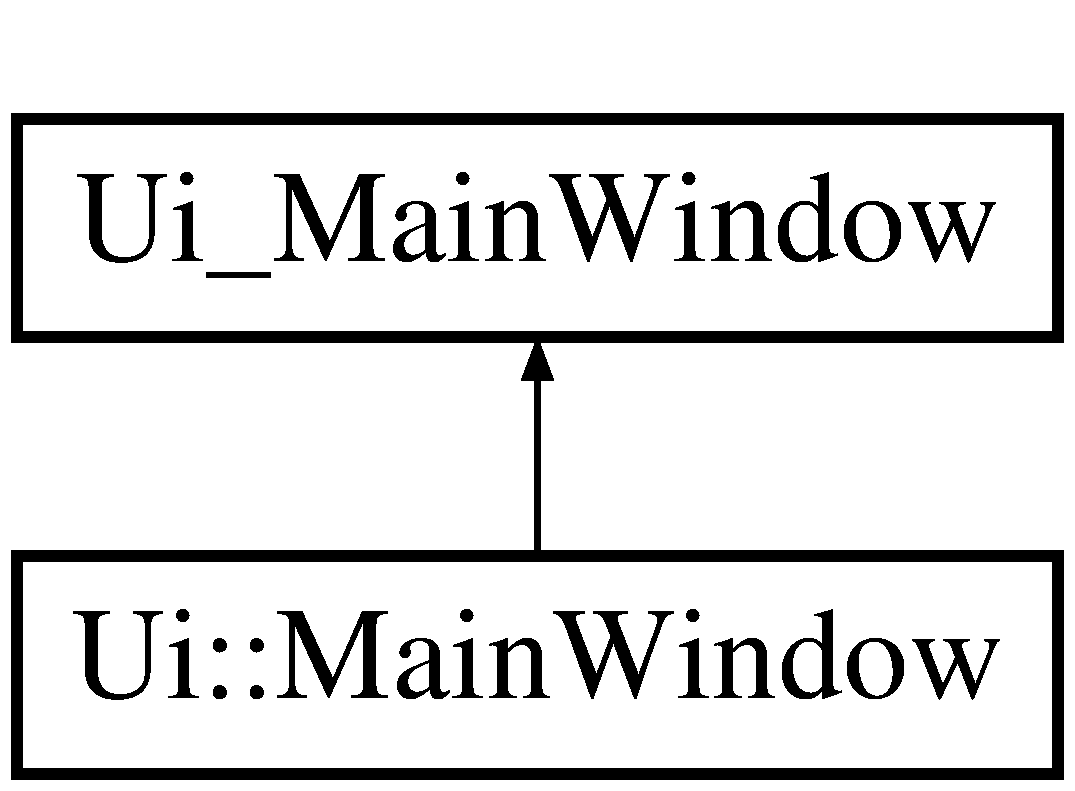
\includegraphics[height=2.000000cm]{class_ui___main_window}
\end{center}
\end{figure}
\subsection*{Public Member Functions}
\begin{DoxyCompactItemize}
\item 
\mbox{\Hypertarget{class_ui___main_window_acf4a0872c4c77d8f43a2ec66ed849b58}\label{class_ui___main_window_acf4a0872c4c77d8f43a2ec66ed849b58}} 
void {\bfseries setup\+Ui} (Q\+Main\+Window $\ast$\mbox{\hyperlink{class_main_window}{Main\+Window}})
\item 
\mbox{\Hypertarget{class_ui___main_window_a097dd160c3534a204904cb374412c618}\label{class_ui___main_window_a097dd160c3534a204904cb374412c618}} 
void {\bfseries retranslate\+Ui} (Q\+Main\+Window $\ast$\mbox{\hyperlink{class_main_window}{Main\+Window}})
\end{DoxyCompactItemize}
\subsection*{Public Attributes}
\begin{DoxyCompactItemize}
\item 
\mbox{\Hypertarget{class_ui___main_window_a30075506c2116c3ed4ff25e07ae75f81}\label{class_ui___main_window_a30075506c2116c3ed4ff25e07ae75f81}} 
Q\+Widget $\ast$ {\bfseries central\+Widget}
\item 
\mbox{\Hypertarget{class_ui___main_window_a5f019495ed714a4c64dd54849b12b87c}\label{class_ui___main_window_a5f019495ed714a4c64dd54849b12b87c}} 
\mbox{\hyperlink{class_g_l_widget}{G\+L\+Widget}} $\ast$ {\bfseries widget}
\item 
\mbox{\Hypertarget{class_ui___main_window_ab96ab0f0578098521fa69a75aa5cdde8}\label{class_ui___main_window_ab96ab0f0578098521fa69a75aa5cdde8}} 
Q\+Widget $\ast$ {\bfseries layout\+Widget}
\item 
\mbox{\Hypertarget{class_ui___main_window_aecd96a04789fcfec3f98d80390ad8184}\label{class_ui___main_window_aecd96a04789fcfec3f98d80390ad8184}} 
Q\+V\+Box\+Layout $\ast$ {\bfseries vertical\+Layout}
\item 
\mbox{\Hypertarget{class_ui___main_window_a6e290c2eca03b98b6f379c71910c0ed6}\label{class_ui___main_window_a6e290c2eca03b98b6f379c71910c0ed6}} 
Q\+Plain\+Text\+Edit $\ast$ {\bfseries plain\+Text\+Edit}
\item 
\mbox{\Hypertarget{class_ui___main_window_ac92cce0478c1025ace05ff4f8870bb1c}\label{class_ui___main_window_ac92cce0478c1025ace05ff4f8870bb1c}} 
Q\+Push\+Button $\ast$ {\bfseries push\+Button\+\_\+3}
\item 
\mbox{\Hypertarget{class_ui___main_window_a59a7d8124bce933d63f53f2153d447b4}\label{class_ui___main_window_a59a7d8124bce933d63f53f2153d447b4}} 
Q\+Push\+Button $\ast$ {\bfseries push\+Button\+\_\+2}
\item 
\mbox{\Hypertarget{class_ui___main_window_adafdad7c065227c5d14b68d75789cbe2}\label{class_ui___main_window_adafdad7c065227c5d14b68d75789cbe2}} 
Q\+Push\+Button $\ast$ {\bfseries push\+Button\+\_\+5}
\item 
\mbox{\Hypertarget{class_ui___main_window_acb0b2f196dc2224f287b67594233297f}\label{class_ui___main_window_acb0b2f196dc2224f287b67594233297f}} 
Q\+Push\+Button $\ast$ {\bfseries push\+Button\+\_\+4}
\item 
\mbox{\Hypertarget{class_ui___main_window_ad332d93084584930878f1daf5f84cdbf}\label{class_ui___main_window_ad332d93084584930878f1daf5f84cdbf}} 
Q\+Push\+Button $\ast$ {\bfseries push\+Button}
\item 
\mbox{\Hypertarget{class_ui___main_window_a2be1c24ec9adfca18e1dcc951931457f}\label{class_ui___main_window_a2be1c24ec9adfca18e1dcc951931457f}} 
Q\+Menu\+Bar $\ast$ {\bfseries menu\+Bar}
\item 
\mbox{\Hypertarget{class_ui___main_window_a5172877001c8c7b4e0f6de50421867d1}\label{class_ui___main_window_a5172877001c8c7b4e0f6de50421867d1}} 
Q\+Tool\+Bar $\ast$ {\bfseries main\+Tool\+Bar}
\item 
\mbox{\Hypertarget{class_ui___main_window_a50fa481337604bcc8bf68de18ab16ecd}\label{class_ui___main_window_a50fa481337604bcc8bf68de18ab16ecd}} 
Q\+Status\+Bar $\ast$ {\bfseries status\+Bar}
\end{DoxyCompactItemize}


The documentation for this class was generated from the following file\+:\begin{DoxyCompactItemize}
\item 
ui\+\_\+mainwindow.\+h\end{DoxyCompactItemize}

%--- End generated contents ---

% Index
\backmatter
\newpage
\phantomsection
\clearemptydoublepage
\addcontentsline{toc}{chapter}{Index}
\printindex

\end{document}
